%\documentclass[11pt,reqno]{amsart}
%%\documentclass[a4paper,10pt]{scrartcl}
%% \oddsidemargin = 1cm
%% \textwidth = 14cm
% \topmargin = -1.0cm
%% \footskip = 3cm
%\usepackage[width=16.0cm, left=2.7cm, height=23cm, top = 2cm]{geometry}

\documentclass[11pt]{amsart}


%\usepackage[paperwidth=400.0pt,paperheight=624.0pt,margin=20.0pt]{geometry}
\usepackage[text={504pt,680pt},centering]{geometry}

\usepackage{lipsum}
\usepackage[english]{babel}
\usepackage{fancyhdr}
\usepackage[utf8]{inputenc} 
\usepackage{setspace}
\usepackage{color}
%\usepackage{refcheck}
\usepackage{amsmath, amsthm, amssymb}
\usepackage{amsfonts}
%\usepackage{showkeys}
\usepackage{enumitem}
%\usepackage[dvips]{epsfig}
\usepackage{graphicx}
\usepackage[english]{babel}
%\usepackage{enumerate}
\usepackage[hidelinks]{hyperref}
%\usepackage{showlabels}
\usepackage{cleveref}
\usepackage{soul}
\usepackage[skip=0.5pt]{caption}
%\usepackage{caption}
\usepackage{subcaption}
\captionsetup[subfigure]{labelformat=empty}

\usepackage[export]{adjustbox}
\usepackage{wrapfig}
\usepackage{float}
\usepackage{graphicx}
\usepackage[mathscr]{euscript}
\usepackage{ulem}
% \usepackage{biblatex}
% \addbibresource{references.bib}
\usepackage{cleveref}



% \theoremstyle{plain}
% \newtheorem{thm}{Theorem}[section]
% \newtheorem{cor}[thm]{Corollary}
% \newtheorem{lem}[thm]{Lemma}
% \newtheorem{conj}[thm]{Conjecture}
% \newtheorem{prop}[thm]{Proposition}
% \newtheorem{claim}[thm]{Claim}

% \theoremstyle{definition}
% \newtheorem{defi}[thm]{Definition}

% \theoremstyle{remark}
% \newtheorem{rem}[thm]{Remark}


% \numberwithin{equation}{section}
% \renewcommand{\theequation}{\thesection.\arabic{equation}}
% \renewcommand{\thefigure}{\thesection.\arabic{figure}}

\pagestyle{fancy}
\fancyhf{}
\fancyhead[RE,RO]{Joaquin Garcia-Suarez}
\fancyhead[LE,LO]{\it{Research Statement }}
\headsep = 0.75cm


\fancypagestyle{firststyle}
{
\fancyhf{}
\fancyhead[RE,RO]{Joaquin Garcia-Suarez}
\fancyhead[LE,LO]{\it{Research Statement }}
\headsep = 0.75cm
}


\newcommand{\X}{\mathfrak{X}}
\newcommand{\de}{\partial}
\newcommand{\on}{\overline{\nabla}}
\newcommand{\fls}{(-\Delta)^s}
\newcommand{\R}{\mathbb{R}}
\newcommand{\C}{\mathbb{C}}
\newcommand{\Z}{\mathbb{Z}}
\newcommand{\N}{\mathbb{N}}
\newcommand{\So}{\mathcal{S}}
\newcommand{\Lo}{\mathcal{L}}
\newcommand{\K}{\mathcal{K}}
\newcommand{\F}{\mathcal{F}}
\newcommand{\eps}{\varepsilon}

\newcommand{\average}{{\mathchoice {\kern1ex\vcenter{\hrule height.4pt
width 6pt depth0pt} \kern-9.7pt} {\kern1ex\vcenter{\hrule
height.4pt width 4.3pt depth0pt} \kern-7pt} {} {} }}
\newcommand{\ave}{\average\int}
\def\R{\mathbb{R}}

\date{}
\author{}

\begin{document}
\thispagestyle{firststyle}
\onehalfspacing


% \begin{center}

% {\LARGE  
% %SNSF Ambizione Call 2022 ---
% J. Garcia-Suarez's Research Statement}
% % \\[0.2cm]
% % {\large\bf }
% \end{center}

% % \vspace{-0.1cm}
% % %\section{Summary}
% \vspace{-0.25cm}
% %\thispagestyle{empty}


\noindent\textbf{\large Vision.}  
%
My group's aim is to \textbf{develop theoretical and computational tools that unlock results previously out of reach} 
%
— like wear forecasting or
%
precise location of acoustic bandgaps — 
%
in technological problems where \textbf{solid and fluid mechanics interact with interfaces and across scales}. 
%
The three themes that will define our research during the \textbf{next five years} are: 
%
(I) interface mechanics; 
%
(II) wave propagation in layered media; 
%
and (III) computational strategies to enable (I) and (II).  

\medskip

\centerline{
\textbf{\large Theme I — Solids and Fluids in Interface Mechanics Across Scales}
}


\noindent \textbf{Interfaces set durability, feel, and failure}: 
%
microscale wear often dictates machinery lifetime; 
%
thin-film lubrication controls whether soft bodies make or avoid contact; 
%
frictional weakening governs rupture of geophysical and mechanical interfaces. 
%
\textbf{Key variables} (e.g., wear volume, contact area and frictional force) \textbf{remain challenging to predict}.  
%
After meaningful contributions, my group has a clear research program that could be funded by competitive government grants or via industry collaborations.   


\begin{figure}[H]
    \centering
    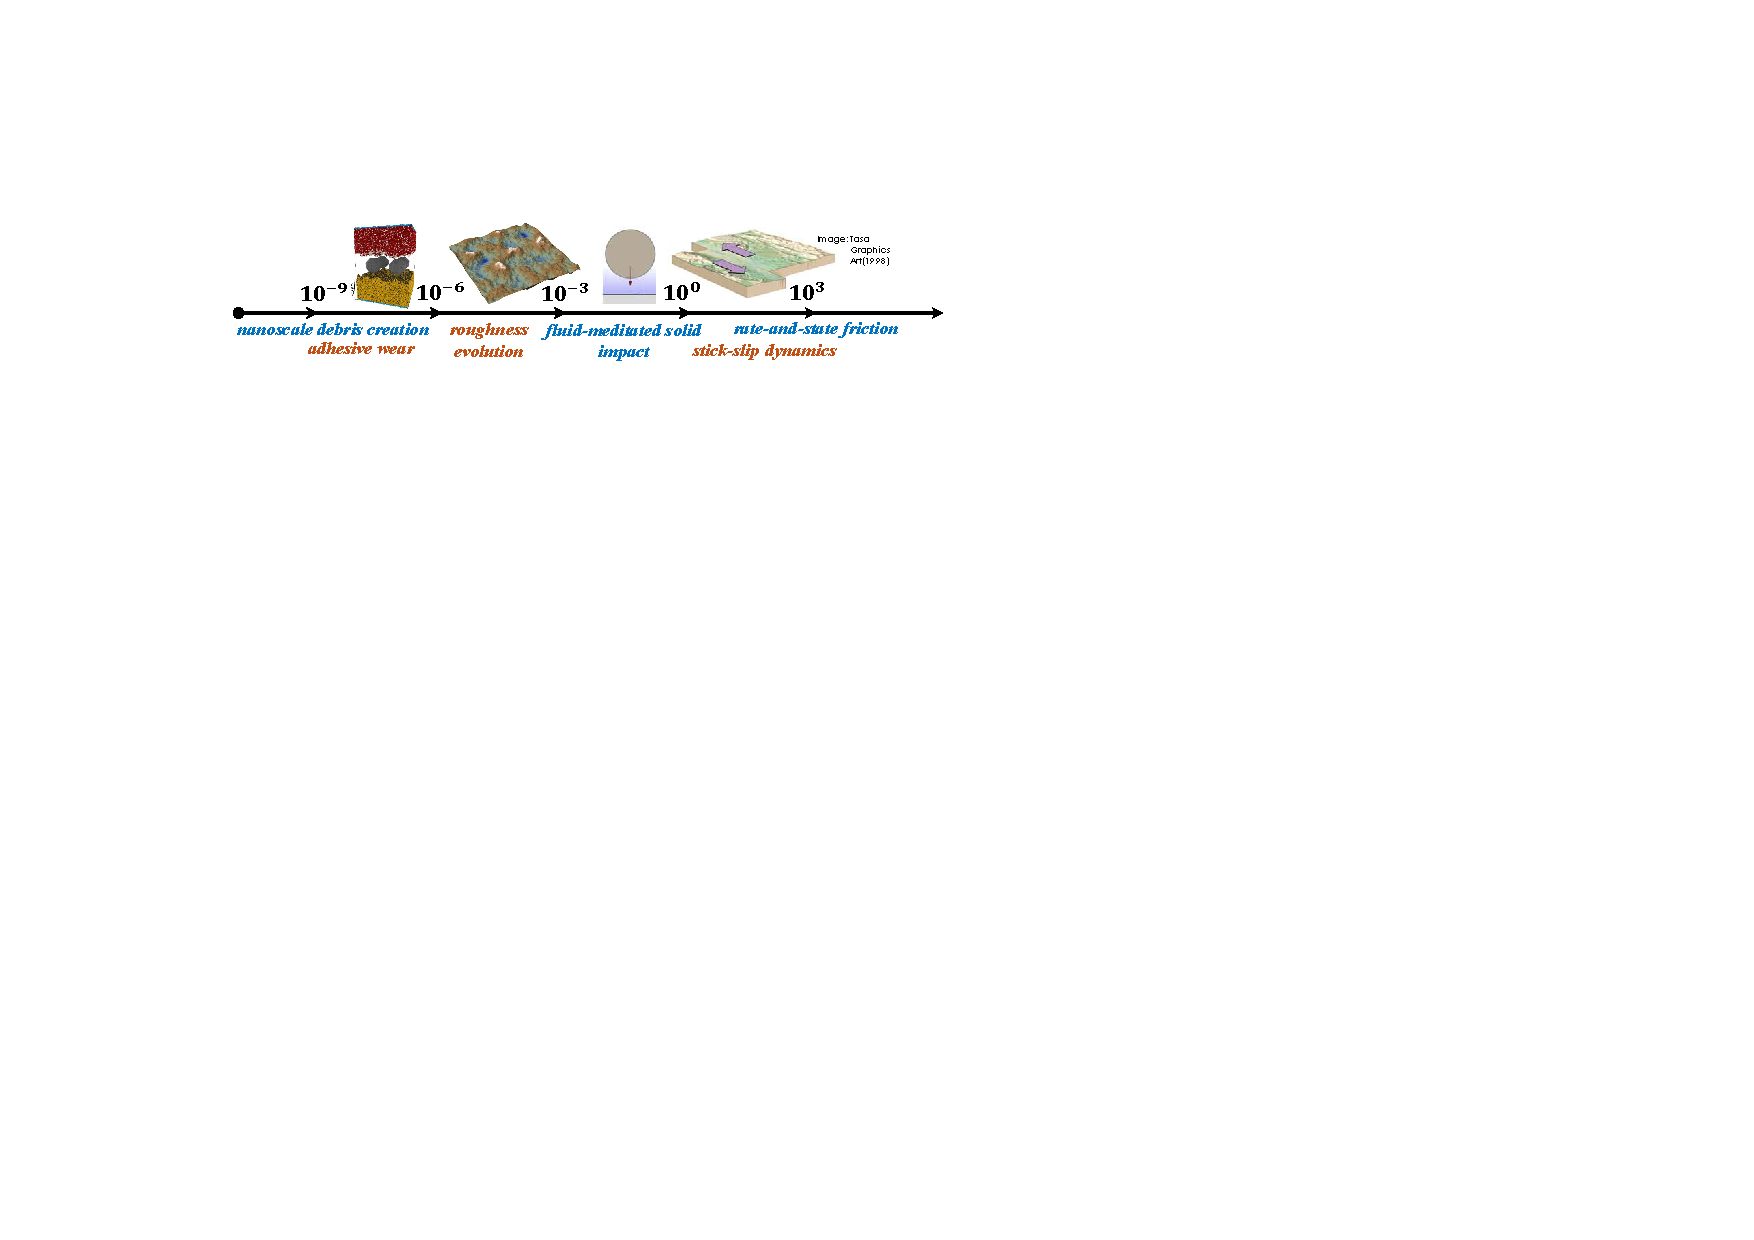
\includegraphics[width=0.995\linewidth]{figures/friction_scales.pdf}
    \captionsetup{width=\textwidth}
    \vspace{-4mm}
    \caption{
    % \centering \it
    Across twelve orders of 
    magnitude in 
    length scales, 
    %
    we utilize molecular dynamics, 
    %
    roughness statistics, 
    %
    elastohydrodynamic lubrication theory, 
    %
    % DEM-FEM coupling, 
    %
    and data-driven friction models 
    %
    to predict wear \cite{ductile_wear}, 
    %
    track surface evolution \cite{Tobias}, 
    %
    control soft contact \cite{Bilotto}, 
    %
    % bridge continuum and granular media, 
    %
    and enable fault rupture simulations \cite{Gaetan}.
    }
\end{figure}

%%%%%%%%%%%%%%%%%%%%%%%%%%%%%%%%%%%%%%%%%%%%%%%%%%
\begin{wrapfigure}{l}{.35\textwidth}
\vspace{-0.5cm}
    \begin{minipage}{\linewidth}
    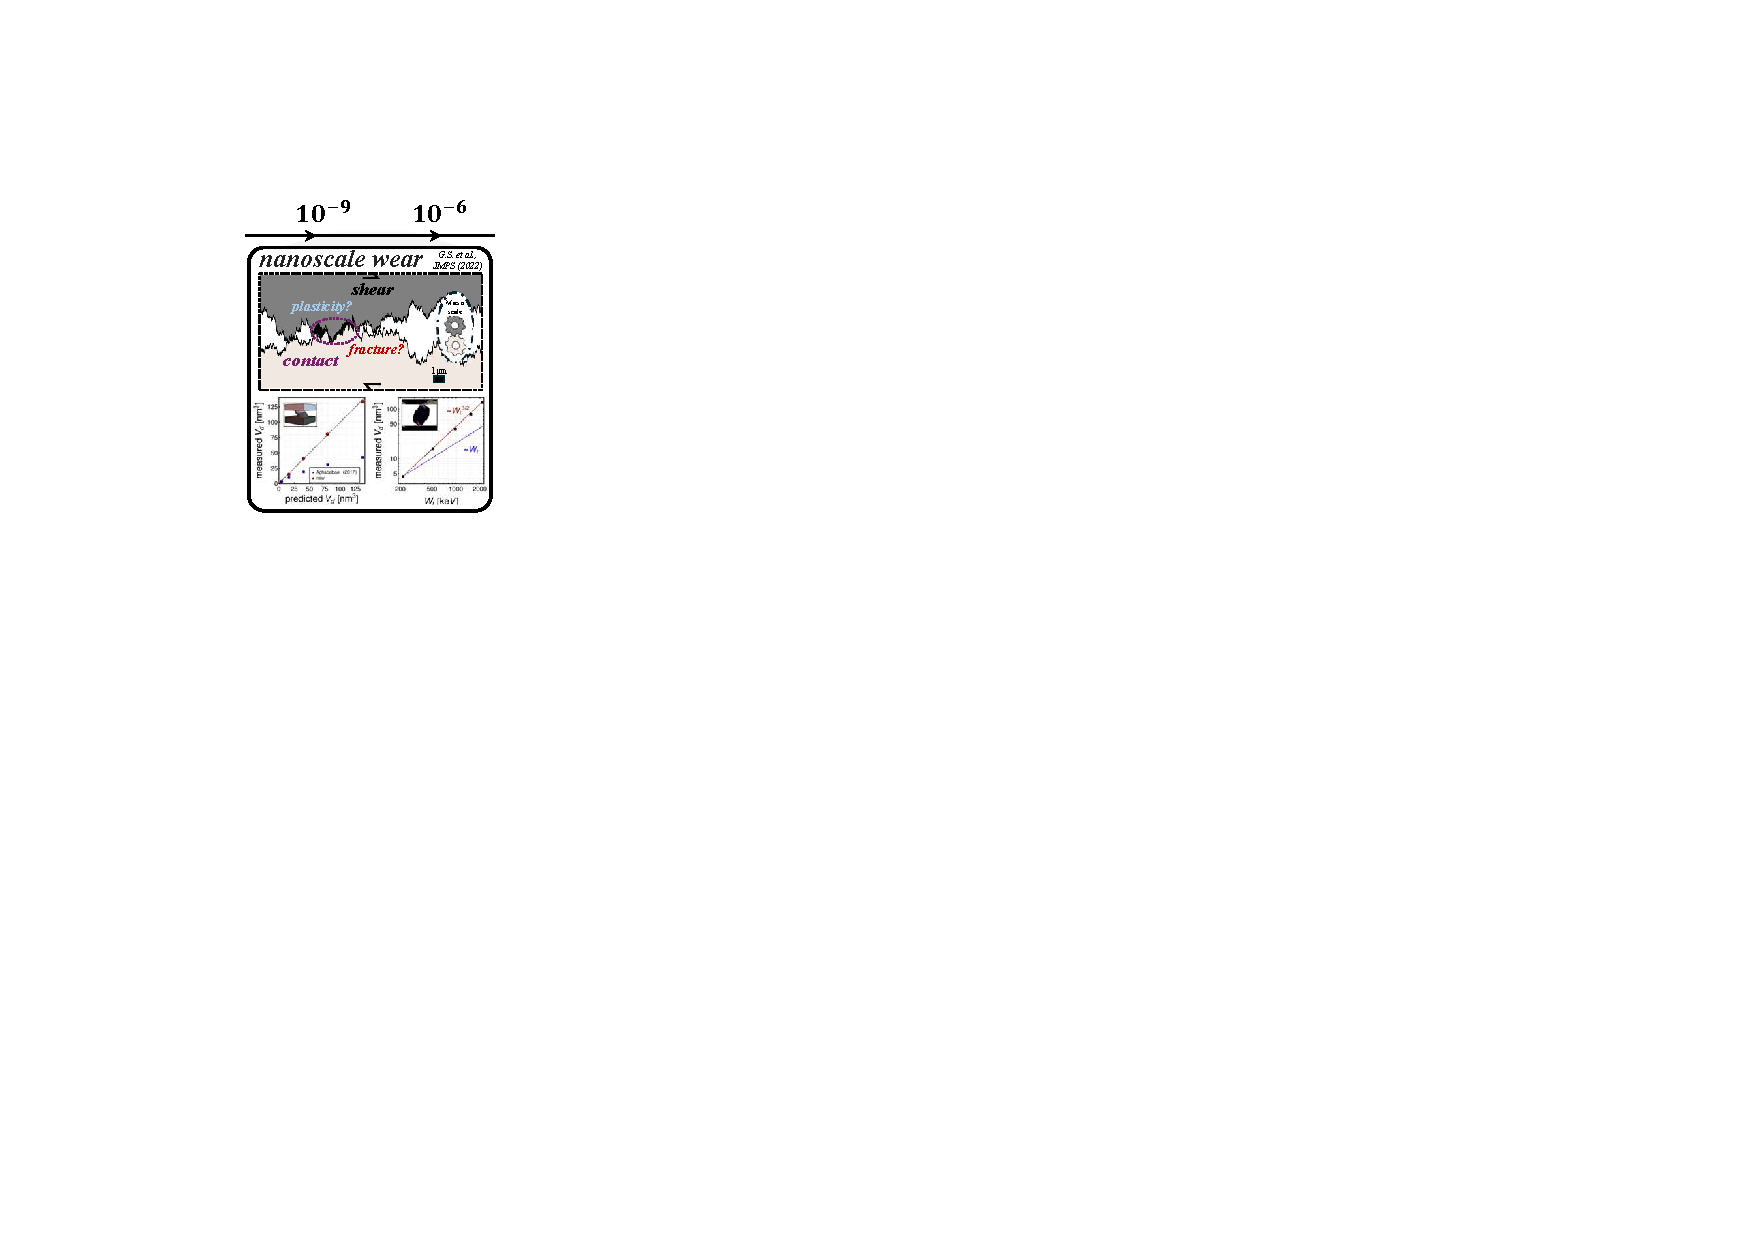
\includegraphics[width=\linewidth]{figures/panel_wear.pdf}
\end{minipage}
\vspace{-0.cm}
\caption{
Scaling change in wear volume v. tangential work: plasticity yields to fracture \cite{ductile_wear}. 
}
\label{fig:panel_wear}
\end{wrapfigure}
At the \textbf{nanoscale} we have used molecular dynamics to resolve two-asperity junction failure \cite{ductile_wear,Sacha}, 
%
then distilled the numerical results into two \textbf{wear-work scaling laws} relating the debris volume $V_d$ and the tangential work to slide $W_t$: 
%
$V_d \sim W_t$ in the small-asperity, plasticity-dominated regime and $V_d \sim W_t^{3/2}$ in the fracture-dominated regime \cite{ductile_wear}, see \cref{fig:panel_wear}. 
%
These findings suggest that nanoscale \textbf{debris creation} can be more \textbf{energetically favorable} than previously assumed. 
%
While macroscale experiments often report an approximately linear relation \cite{ramin_wear}, our next objective is to reconcile the apparent cross-scale mismatch by showing that this linearity arises not from a different failure mechanism but from the geometry and statistics of \textbf{random rough surfaces} \cite{Persson}. 
%
At AnyU, this program would benefit greatly from interactions with  (for reliability/lifetime \cite{friction_cost}) and with members of the  such as Profs. X and Y (to deepen the nanomechanical aspects) and Z (consider influence of oxidation).
% and Henann (micro and mesoscale wear).
%%%%%%%%%%%%%%%%%%%%%%%%%%%%%%%%%%%%%%%%%%%%%%%%%%

\medskip

%%%%%%%%%%%%%%%%%%%%%%%%%%%%%%%%%%%%%%%%%%%%%%%%%%
For \textbf{soft solids interacting with a surface through a thin fluid layer} \cite{Rallabandi}, 
%
I coupled lubrication theory to solid inertia and deformations to derive a \textbf{governing dimensionless group} $\phi$ --  the ratio between the characteristic time of viscous pre-contact drainage and the time required for elastic waves to traverse the leading edge -- 
that \textbf{classifies the regimes of fluid-mediated normal impact} of compliant solids (and of droplets) \cite{Bilotto}:  
%
for 
$\phi \ll 1$ the response is quasi-static -- inertia can be neglected, elasticity dominates -- and only a small air bubble is entrapped;
for 
$\phi \sim 1$ inertia and elasticity compete, producing delayed touchdown leading to maximum air entrainment;
for 
$\phi \gg 1$ local deceleration -- inertia -- dominates, small bubbles form. 

\begin{wrapfigure}{r}{.35\textwidth}
\vspace{-0.1cm}
    \begin{minipage}{\linewidth}
    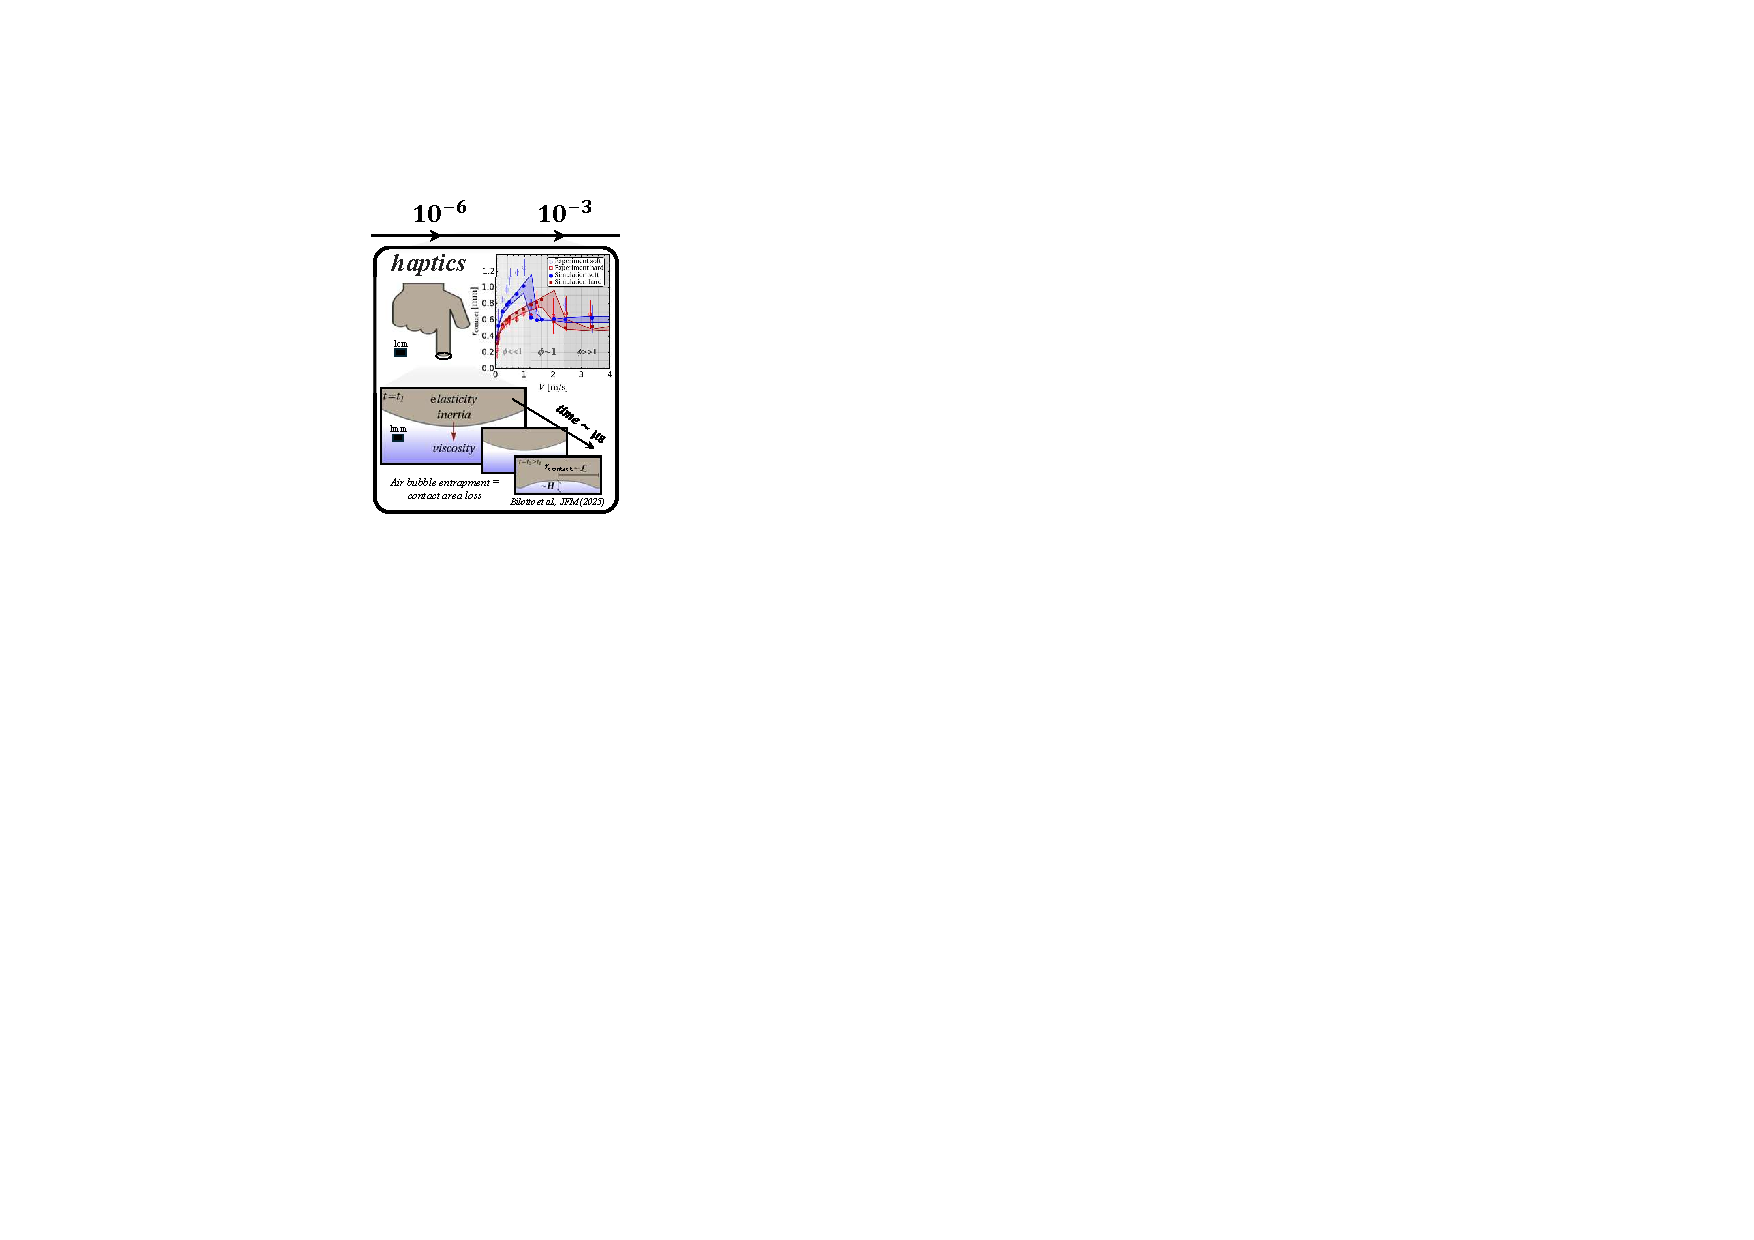
\includegraphics[width=\linewidth]{figures/panel_haptics.pdf}
\end{minipage}
\vspace{-0.cm}
\caption{
Fluid-mediated approach of soft solid (fingertip) to rigid surface ($r_{contact}>0$) \cite{Bilotto}.
}
    \label{fig:panel_haptics}
\end{wrapfigure}
%
\noindent Experiments -- supported by our numerical simulations -- exhibit these three regimes, as shown in \cref{fig:panel_haptics}: the framework explains the \textbf{evolution of the bubble’s characteristic dimensions}, both vertical ($\mathcal{H}$) and radial ($\mathcal{L}$), the latter corresponding directly to the experimentally measured contact radius $r_{\text{contact}}$.   
%
This scaling unifies a wide range of observations -- across solid and droplet impact -- and provides a predictive map for dynamic contact area optimization for soft solids. 
%
I am now examining \textbf{how air entrainment can be suppressed} by geometry and surface curvature  \cite{Arxiv}, aiming for a broader framework of how fluid–structure interaction (FSI) governs contact formation. 
%
This mechanics also determines the \textbf{haptic forces} that develop during the pre-contact squeeze phase \cite{haptics} and the porosity patterns observed in \textbf{inkjet bioprinting} \cite{bioprinting}. 
%
I anticipate collaborations with Prof. I on theoretical aspects, Prof. II on analysis of low-Re flows coupled to rough surfaces, Profs. III and IV on high-fidelity FSI simulations, as well as with Prof. IV on the theory of adhesion and contact experiments in soft materials. 
%


\medskip

%%%%%%%%%%%%%%%%%%%%%%%%%%%%%%%%%%%%%%%%%%%%%%%%%%

\begin{wrapfigure}{l}{.35\textwidth}
\vspace{-0.5cm}
    \begin{minipage}{\linewidth}
    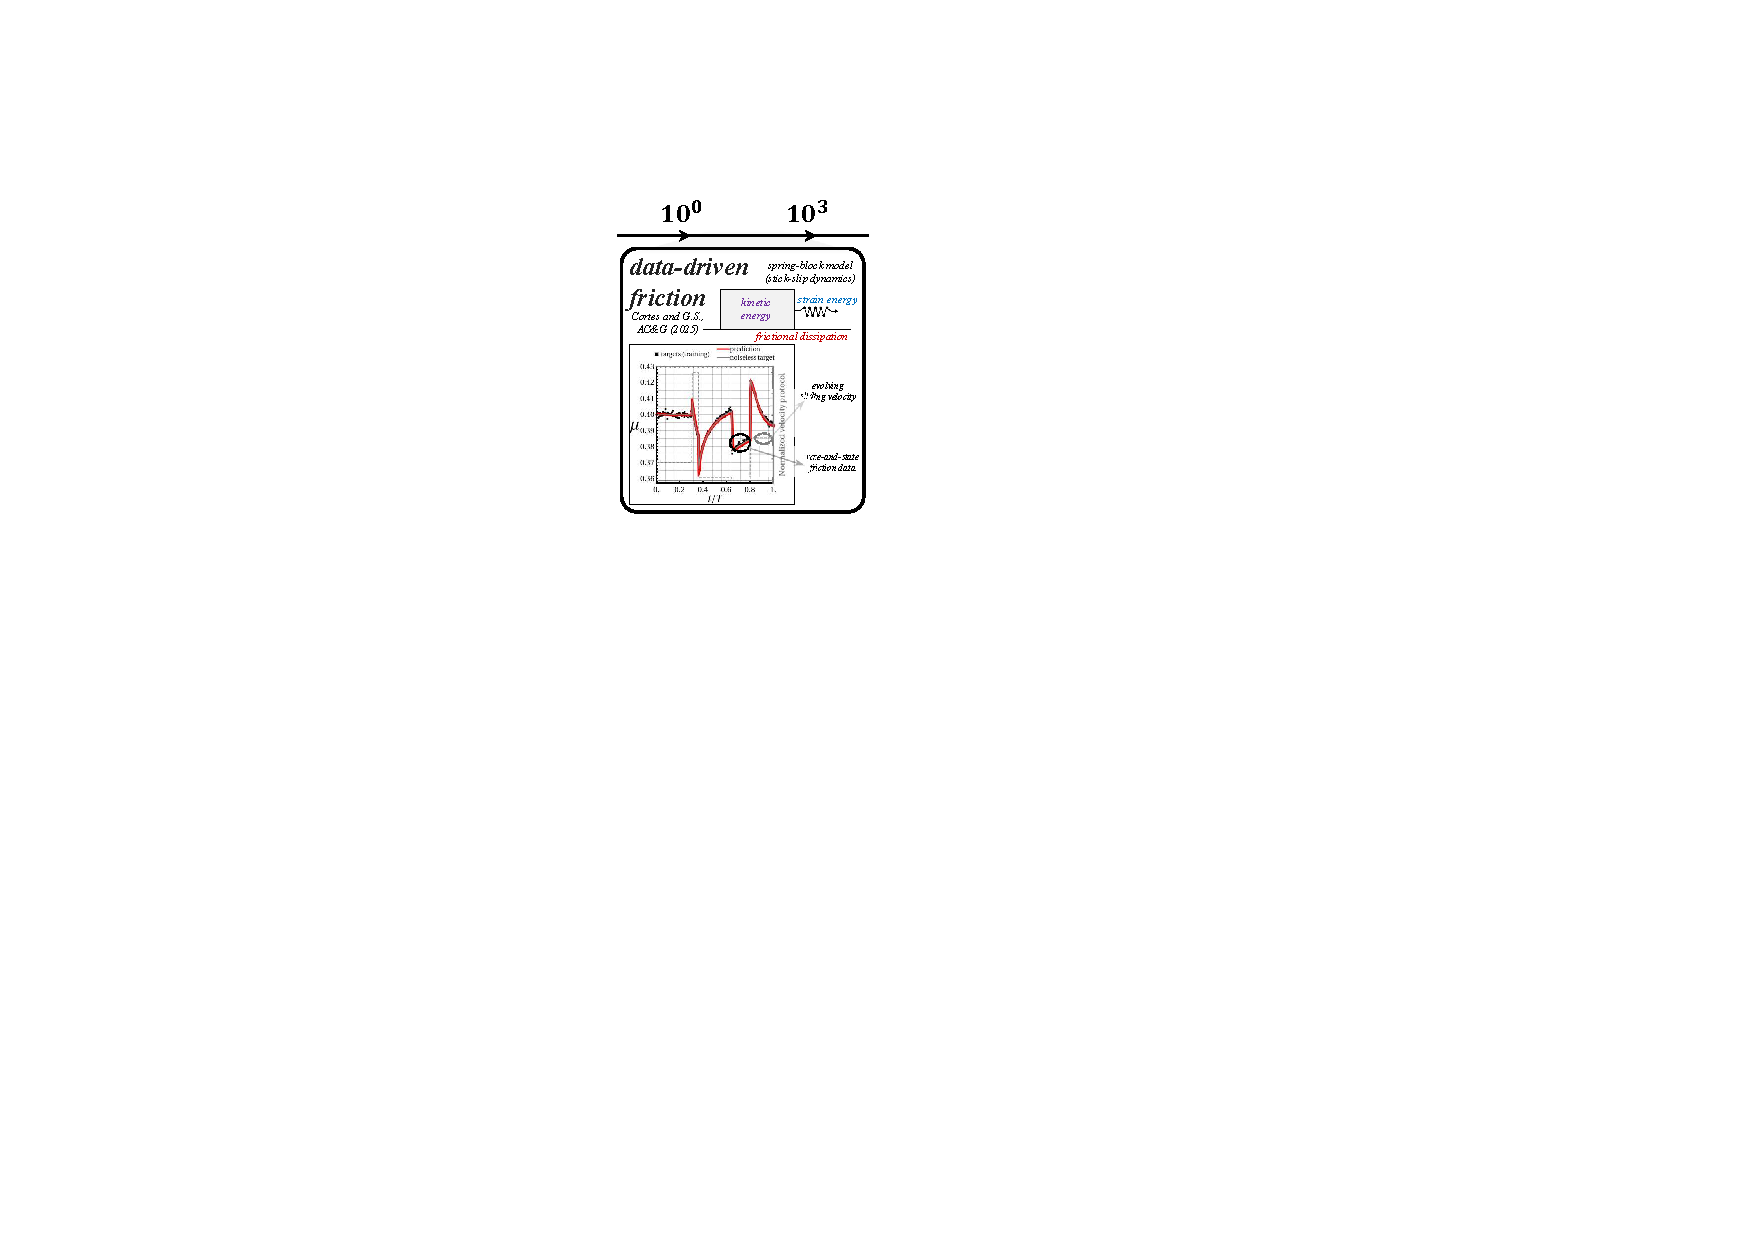
\includegraphics[width=\linewidth]{figures/panel_DDCF_v2.pdf}
    \label{fig:panel_DDCF}
\end{minipage}
\vspace{-0.5cm}
\caption{
Current work (funded by SNSF Ambizione project) focused on developing data-driven, machine-learned friction models \cite{Gaetan}.
}
\end{wrapfigure}
In the context of \textbf{dynamic rupture}, my team is developing \textbf{data-informed friction laws} that are constrained by laboratory observations \cite{Gaetan}. 
%
These models provide an alternative to the limited heuristic formulations currently used in large-scale simulations of fault slip.
%
By blending machine learning (ML) with rate-and-state theory, we aim to capture the complexity of real frictional history dependence with velocity weakening and strengthening.  
%
The broader goal is to translate recent advances in machine learning into \textbf{tools that serve the needs of geophysicists and mechanical engineers} \cite{Batista}, where friction often limits predictive accuracy in simulations ranging from fault slip to thin-film molecular lubrication. 
%

\newpage

\centerline{
\textbf{\large Theme II — Wave Propagation in Heterogeneous Media: One Math, Many Physics}
}

\noindent Layered media underpin \textbf{photonic, phononic and acoustic} devices; 
%
all require robust bandgap placement and broadband transmission or absorption;  
%
achieving this is traditionally left to brute-force evolutionary inverse design methods. 
% that scan the design space in search of layerings that deliver the desired performance. 
%
Forward predictions are run using the \textbf{transfer matrix method (TMM)}, a numerical \textbf{black-box} lacking both a bridge between wave physics and performance, and a tractable means of uncertainty quantification (UQ) beyond costly Monte Carlo. 
%
% Uncertainty quantification (UQ) to map manufacturing tolerances to potential performance losses also heavily rely on TMM runs in the order of thousands, at least.  
%
Since my PhD, I have been developing an \textbf{alternative to TMM} exploiting the group-theoretic structure of transfer matrices (see top panel of \cref{fig:waves_panels}): 
%
\textbf{a physics-agnostic prediction framework} that spans electrons, light, elastic and acoustic waves, 
%
% enables idea transfer and inverse design.
\textbf{based on a Lie-group approach to wave propagation in layered media} that has already yielded a key result: the harmonic decomposition of transfer matrices \cite{JMPS}. 
%
The latter enables closed-form expressions, e.g., for the Bloch discriminant of band edges and slab's transmission/reflection coefficients.

% \vspace{3mm}

\begin{wrapfigure}{r}{.35\textwidth}
\vspace{-0.1cm}
    \begin{minipage}{\linewidth}
    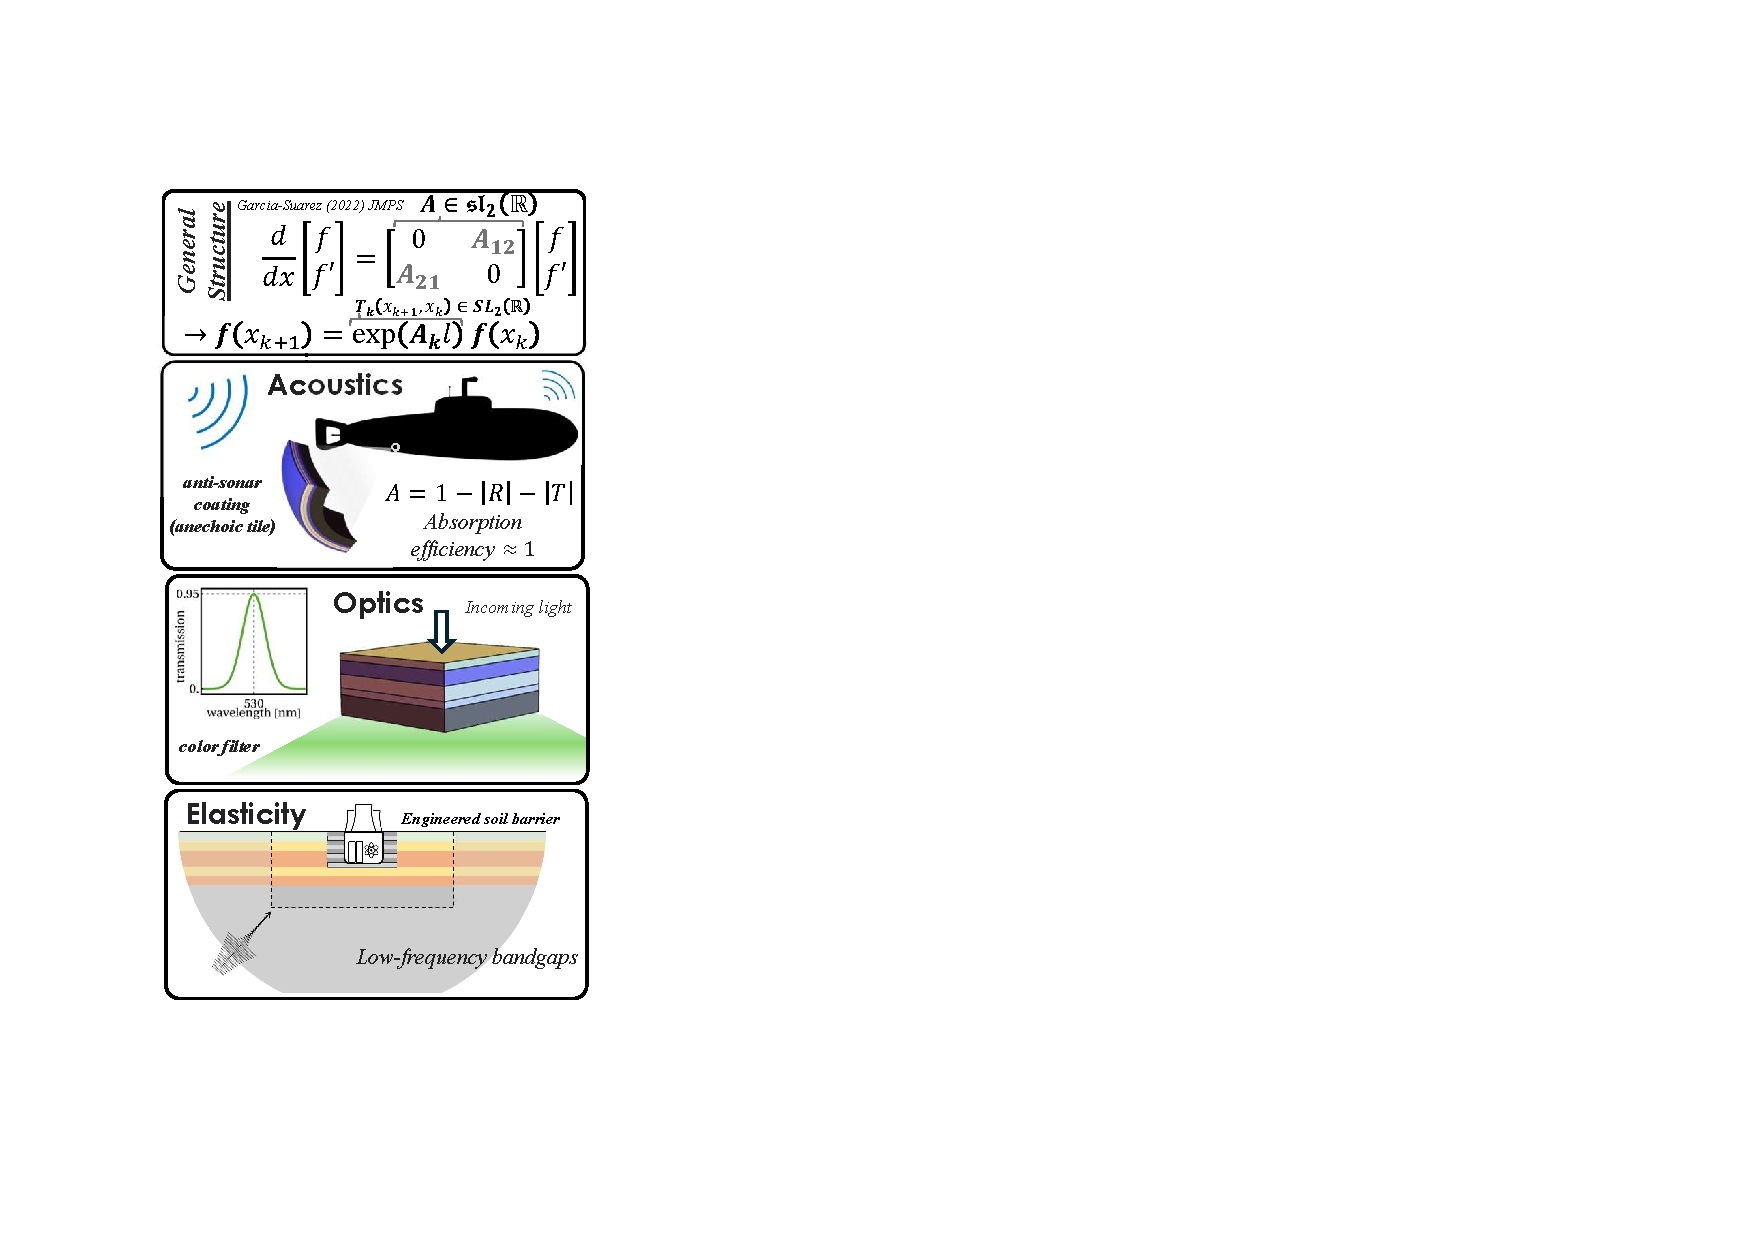
\includegraphics[width=\linewidth]{figures/waves_panels.pdf}
\end{minipage}
\vspace{-0.cm}
\caption{Group-theoretic physics-agnostic framework to design structures for acoustic, electromagnetic and elastic wave control \cite{JMPS}. 
}
    \label{fig:waves_panels}
    \vspace{-0.6cm}
\end{wrapfigure}
The same math -- up to relabeling of the physical variables and parameters -- models a \textbf{variety of applications}: broadband acoustic absorption in anechoic tiles, light wavelength selective transmission for color filters, and elastic bandgaps for vibration isolation \cite{EJM_Javi}, see \cref{fig:waves_panels}. 
%
In contrast with the current state-of-the-art \cite{Morrison}, the decomposition's structure opens the door to \textbf{GPU-bound second-order optimization} in all those areas. 
%
We are \textbf{expanding the key result} from 2x2 matrices to 4x4 to capture waves in composite Euler-Bernouilli beams \cite{Nur} that can serve as waveguides. 
%
My team will focus next on including \textbf{viscoelastic layers and inclined waves}, 
%
and couple to surrounding fluids to design underwater/air absorbers with flat, wide transmission plateaus under mass and fabrication constraints. 
%


% \vspace{5mm}
\newpage

\centerline{
\textbf{\large Theme III — Methods Development (supports I–II)}
}


\noindent We develop methods as needed to \textbf{address specific problems} \cite{d-ref,PSI}. 
%
For instance, in FSI, I am developing compact, physics-based Python scripts (adapted from \cite{Repo}) for \textbf{elastohydrodynamic lubrication simulations of elastic solids} \cite{EHL_GH}. 
%
The current model combines an axisymmetric Reynolds equation with a Green’s function–based elastic response in dimensionless form, which can easily handle different shapes, and upcoming work will extend it to include dissipative rebounds, viscoelasticity, and 2D roughness effects.
%

\newpage

\thispagestyle{plain}
\pagenumbering{gobble}
%\printbibliography
%\bibliography{references}
%\bibliographystyle{plain}
% \bibliography{references}
% \bibliographystyle{acm}

% \renewcommand\refname{References}  


\section*{References}

\vspace{0.25cm}
\begingroup
\renewcommand{\section}[2]{}%
\begin{thebibliography}{99}

    \bibitem[1]{ductile_wear}
	\newblock \textbf{Garcia-Suarez, J.}, Brink, T., Molinari, J.-F. (2023)
	\newblock ``Breakdown of Reye's theory in nanoscale wear''.
	\newblock \textit{Journal of the Mechanics and Physics of Solids}.

    \bibitem[2]{Tobias}
	\newblock \textbf{Garcia-Suarez, J.}, Brink, T., Molinari, J.-F. (2024)
	\newblock ``Roughness evolution induced by third-body wear''.
	\newblock \textit{Tribology Letters}.

    \bibitem[3]{Bilotto}
	\newblock Bilotto, J., Kolinski, J., Lecampion, B., Molinari, S., Subhash, G., \textbf{Garcia-Suarez, J.} (2024)
	\newblock ``Fluid-mediated impact of soft solids''. 
	\newblock \textit{Journal of Fluid Mechanics}.

    \bibitem[4]{Gaetan}
    \newblock Cortes, G., and \textbf{Garcia-Suarez, J.} (2025)
    \newblock ``Data-driven dynamic friction models based on Recurrent Neural Networks'',
    \newblock \textit{Applied Computing and Geosciences}.

    \bibitem[5]{Sacha}
	\newblock Wattel, S., \textbf{Garcia-Suarez, J.}, Molinari, J.-F. (2022)
	\newblock ``Understanding the mechanisms of adhesive wear for heterogeneous materials through atomistic simulations'', 
	\newblock \textit{Extreme Mechanics Letters}.

    \bibitem[6]{ramin_wear}
	\newblock Aghababaei, R., Wagner, D., Molinari, J.-F. (2017)
	\newblock ``On the debris-level origins of adhesive wear'',
	\newblock \textit{Proceedings of the National Academy of Sciences}. 

    \bibitem[7]{Persson}
	\newblock Xu, Y., Li, X., Chen, Q., Zhou, Y. (2024)
	\newblock ``Persson’s theory of purely normal elastic rough surface contact: a tutorial based on stochastic process theory'', 
	\newblock \textit{International Journal of Solids and Structures}. 

    \bibitem[8]{friction_cost}
	\newblock Holmberg, K., Erdemir, A. (2017)
	\newblock ``Influence of tribology on energy consumption, costs and emission''.
	\newblock \textit{Friction}.
    

    \bibitem[9]{Rallabandi}
	\newblock Rallabandi, B. (2024)
	\newblock ``Fluid-elastic interactions near contact at low Reynolds number'',  
	\newblock \textit{Annual Review of Fluid Mechanics}.

    \bibitem[10]{Arxiv}
	\newblock \textbf{Garcia-Suarez, J.}
	\newblock ``A matter of shape: contact area optimization in soft lubrication'',
	\newblock Submitted to \textit{Tribology letters} (arXiv:2411.04641).

    
    \bibitem[11]{haptics}
    \newblock Wiertlewski, M., Fenton Friesen, R., and Colgate, J. E. (2016)
    \newblock ``Partial squeeze film levitation modulates fingertip friction'',
    \newblock \textit{Proceedings of the National Academy of Sciences}.
    % DOI: 10.1073/pnas.1603908113

    \bibitem[12]{bioprinting}
    \newblock Derby, B. (2012)
    \newblock ``Printing and prototyping of tissues and scaffolds'',
    \newblock \textit{Science}. 
    % https://doi.org/10.1126/science.1226340

    \bibitem[13]{Batista} 
    \newblock Carlson, J. M., and Batista, A. A. (1996)
    \newblock ``Constitutive relation for the friction between lubricated surfaces'',
    \newblock \textit{Physical Review E}.
    % DOI: 10.1103/PhysRevE.53.4153
    
    \bibitem[14]{JMPS}
	\newblock \textbf{Garcia-Suarez, J.} (2022)
	\newblock ``Harmonic decomposition of the trace of 1D transfer matrices in layered media''.
	\newblock \textit{Journal of the Mechanics and Physics of Solids}.

    \bibitem[15]{EJM_Javi}
	\newblock Gonz\'{a}lez-Carbajal, J., Lemm, M., \textbf{Garcia-Suarez, J.} (2024)
	\newblock ``On the lowest-frequency bandgap of 1D phononic crystals''.
	\newblock \textit{European Journal of Mechanics - A/Solids}.

    \bibitem[16]{Morrison}
    \newblock Morrison, N., Pan, S., and Ma, E. Y.
    \newblock ``Physics-agnostic inverse design using transfer matrices'',
    \newblock \textit{APL Machine Learning}.
    % DOI: 10.1063/5.0201234


    \bibitem[17]{Nur}
	\newblock Sangiorgio, N., \textbf{Garcia-Suarez, J.} (2025)
	\newblock ``Harmonic decomposition of transfer matrices for bending waves'',
	\newblock To be submitted to \textit{Journal of the Mechanics and Physics of Solids} (in preparation). 

    \bibitem[18]{d-ref}
	\newblock Wattel, S., Molinari, J.-F., Ortiz, M., \textbf{Garcia-Suarez, J.} (2023) 
	\newblock ``Mesh d-refinement: a data-based computational framework to account for complex material response''. 
	\newblock \textit{Mechanics of Materials}.


    \bibitem[19]{PSI}
	\newblock Cortes, G., Sangiorgio, N.,  \textbf{Garcia-Suarez, J.} (2024) 
	\newblock ``Phase-space iterative solvers''. 
	\newblock Submitted to \textit{Computational Mechanics} (arxiv 2309.14031).
 

    \bibitem[20]{Repo}
    \newblock Bertin, V.
    \newblock \texttt{elastohydrodynamic-bouncing},  
    \newblock GitHub repository, {https://github.com/vincent-bertin/elastohydrodynamic-bouncing} (accessed 2025-11-13).

    \bibitem[21]{EHL_GH}
    \newblock \textbf{Garcia-Suarez, J.}
    \newblock \texttt{soft-contact},  
    \newblock GitHub repository, {https://github.com/jgarciasuarez/soft-contact} (accessed 2025-11-14).

    % \bibitem[111]{bioprinting}
    % \newblock Li, X., Liu, B., Pei, B., Chen, J., Zhou, D., Peng, J., Zhang, X., Jia, W., and Xu, T. (2020)
    % \newblock \textit{Inkjet bioprinting of biomaterials},
    % \newblock \textit{Chemical Reviews}



    
    



     % BURIED STRUCTURES
 %    \bibitem[1]{IJNAG}
	% \newblock \textbf{Garcia-Suarez, J.}, Asimaki, D. (2020)
	% \newblock ``Exact seismic response of smooth rigid retaining walls resting on stiff soil''. 
	% \newblock \textit{International Journal for Numerical and Analytical Methods in Geomechanics}.  

 %        \bibitem[2]{JMPS_ortiz}
	% \newblock \textbf{Garcia-Suarez, J.}, Ortiz, M., Asimaki, D. (2021)
	% \newblock ``Applications of the J-integral to dynamical problems in geotechnical engineering''. 
	% \newblock \textit{Journal of the Mechanics and Physics of Solids}.

        % NATURAL STRUCTURES
 %        \bibitem[3]{Andrea}
	% \newblock Donnellan, A., \textbf{Garcia‐Suarez, J.}, McPhillips, D., Asimaki, D., Goulet, C., Meng, X., Devine, S., Lyzenga, G. (2022)
	% \newblock ``Toppling of a Trona Pinnacles Spire following the Mw 5.5 Ridgecrest Aftershock of June 2020''.
	% \newblock \textit{Seismological Research Letters}.

 %        \bibitem[4]{Devin}
	% \newblock \textbf{Garcia‐Suarez, J.}, McPhillips, D., Asimaki, D. (expected in 2025)
	% \newblock ``Seismic response and structural integrity evolution of rock towers at Trona, California''.
	% \newblock To be submitted to \textit{Bulletin of the Seismological Society of America}.
        % 1D-SRA

 %    \bibitem[5]{geotechnique-1}
	% \newblock \textbf{Garcia‐Suarez, J.}, Seylabi, E., Asimaki, D. (2021)
	% \newblock ``Seismic harmonic response of inhomogeneous soil: scaling analysis'',
	% \newblock \textit{Géotechnique}.    

 %    \bibitem[8]{Stiffnessless}
	% \newblock \textbf{Garcia‐Suarez, J.}, Seylani, E., Asimaki, D.
	% \newblock \textit{Linear one-dimensional site response analysis in the presence of stiffness-less free surface for certain power-law heterogeneities},
	% \newblock Soil Dyn. Earthquake Eng. (2021).

 %    \bibitem[6]{DDNSR}
	% \newblock \textbf{Garcia-Suarez, J.}, Cornet, A., Wattel, S., Molinari, J.-F. (2023)
	% \newblock ``Data‐driven 1D wave propagation for site response analysis''.
	% \newblock \textit{International Journal for Numerical and Analytical Methods in Geomechanics}.

 %    \bibitem[7]{geotechnique_2}
	% \newblock \textbf{Garcia‐Suarez, J.}, Seylabi, E., Asimaki, D. (2022)
	% \newblock ``Application of ray methods to one-dimensional site response of inhomogeneous soil deposits''.
	% \newblock \textit{Géotechnique}.
            
 %    \bibitem[8]{Fundamental}
	% \newblock \textbf{Garcia‐Suarez, J.}, Asimaki, D. (2020)
	% \newblock ``On the fundamental resonance mode of inhomogeneous soil deposits''.
	% \newblock \textit{Soil Dynamics and Earthquake Engineering}.
    

	
 %    \bibitem[11]{SDEE_Javi}
	% \newblock \textbf{Garcia-Suarez, J.}, Gonz\'{a}lez-Carbajal, J., Asimaki, D. (2022)
	% \newblock ``Analytical 1D transfer functions for layered soils''.
	% \newblock \textit{Soil Dynamics and Earthquake Engineering}.

 %    \bibitem[12]{Aki_Richards}
	% \newblock Aki, K., Richards, P. (2002)
	% \newblock ``Quantitative Seismology'' 2nd edition.
	% \newblock University Science Books.
    

 %    \bibitem[15]{metafoundation}
	% \newblock Elshazly, F., Seylabi, E. (2023)
	% \newblock ``On seismic isolation of soil-meta-foundation-structure systems''.
	% \newblock \textit{Computers \& Geotechnics}.

 %    \bibitem[16]{Elnaz}
	% \newblock Albers, D., Blancquart, P., Levine, M., Seylabi, E., Stuart, A. (2019)
	% \newblock ``Ensemble Kalman filter methods with constraints''.
	% \newblock \textit{Inverse Problems}.

 %    \bibitem[17]{Silva}
	% \newblock Silva, A., Monticone, F., Castaldi, G., Galdi, V., Alù, A., Engheta, N. (2014)
	% \newblock ``Performing mathematical operations with metamaterials'',
	% \newblock \textit{Science}.

    



    
 %    \bibitem[22]{Manon_1}
	% \newblock Voisin--Leprince, M., \textbf{Garcia-Suarez, J.}, Anciaux, G, Molinari, J.-F. (2022)
	% \newblock ``Finite element method–discrete element method bridging coupling for the modeling of gouge''.
	% \newblock \textit{International Journal for Numerical Methods in Engineering.}

 %    \bibitem[23]{Manon_2}
	% \newblock Voisin--Leprince, M., \textbf{Garcia-Suarez, J.}, Anciaux, G, Molinari, J.-F. (2024)
	% \newblock ``Two-scale concurrent simulations for crack propagation using FEM–DEM bridging coupling''.
	% \newblock \textit{Computational Particle Mechanics.}



 %    \bibitem[26]{Scott}
	% \newblock Sobarzo, J.C., Waitukaitis, S. (2024)
	% %Lyons, J., Sayeed, Z., Anoushiravani, A., Iorio, R.
	% \newblock ``Multiple charge carrier species as a possible cause for triboelectric cycles''.
	% \newblock \textit{Physical Review E}.

 %    \bibitem[27]{nanogenerators}
	% \newblock Cheng, T., Shao, J., Wang, Z.L. (2023)
	% %Lyons, J., Sayeed, Z., Anoushiravani, A., Iorio, R.
	% \newblock ``Triboelectric nanogenerators''.
	% \newblock \textit{Nature Review Methods Primer}.

 %    \bibitem[31]{Liu}
	% \newblock Liu, B., Ortiz, M., Cirak, F. (2024)
	% \newblock ``Towards quantum computational mechanics''.
	% \newblock \textit{Computer Methods in Applied Mechanics and Engineering}.
        
 %    \bibitem[32]{Bessa}
	% \newblock Mozaffar, M., Bostanabad, R., Chen, W., Ehmann, K., Cao, J., Bessa, M. (2019)
	% \newblock ``Deep learning predicts path-dependent plasticity''.
	% \newblock \textit{Proceedings of the National Academy of Sciences}.
 
 %    \bibitem[33]{Trent}
	% \newblock Kirchdoerfer, T., Ortiz, M. (2016)
	% \newblock ``Data-driven computational mechanics''.
	% \newblock \textit{Computer Methods in Applied Mechanics and Engineering}.

    
    

 %    \bibitem[36]{RSF-RNN}
	% \newblock \textbf{Garcia-Suarez, J.} 
	% \newblock ``Data-driven dynamic friction models based on recurrent neural networks''. 
	% \newblock Submitted to \textit{Applied Computing \& Geosciences} (arXiv 2402.14148).

 %    \bibitem[37]{Geubelle}
	% \newblock Geubelle, P., Rice, J. (1995)
	% \newblock ``A spectral method for three-dimensional elastodynamic fracture problems''. 
	% \newblock \textit{Journal of the Mechanics and Physics of Solids}.


 %    \bibitem[38]{Conti}
	% \newblock Conti, S., M{\"u}ller, S., Ortiz, M. (2018)
	% \newblock ``Data-driven problems in elasticity''. 
	% \newblock \textit{Archive for Rational Mechanics and Analysis}.

 %    \bibitem[39]{Hess}
	% \newblock Tauzin, G., Lupo, U., Tunstall, L., Burella Pérez, J., Caorsi, M., Medina-Mardones, A., Dassatti, A., Hess, K. (2021)
	% \newblock ``giotto-tda:: A topological data analysis toolkit for machine learning and data exploration''. 
	% \newblock \textit{Journal of Machine Learning Research}.

    


		%\vspace{2mm}


	
	

	
% 		\vspace{0mm}
% \bibitem[7]{multi_scale_ML}
% 	\newblock Kovachki, N., Liu, B., Sun, X., Zhou, H., Bhattacharya, K., and Ortiz, M., Stuart, A.
% 	\newblock \textit{Multiscale modeling of materials: Computing, data science, uncertainty and goal-oriented optimization},
% 	\newblock MecMat (2021).
	
% 	\vspace{0mm}
% 	\bibitem[13]{Manon}
% 	\newblock Voisin-Leprince, M., \textbf{Garcia-Suarez, J.}, Anciaux, G., Molinari, J.-F.
% 	\newblock \textit{FEM-DEM bridging coupling for the modeling of gouge},
% 	\newblock Int. J. Num. Met. Eng. (2022).
	
	

	
	

		

%	
%	
%*****
%\vspace{0mm}
%\bibitem[FS20]{FS19}
%	\newblock X. Fern\'andez-Real, J. Serra,
%	\newblock \textit{Regularity of minimal surfaces with lower dimensional obstacles},
%	\newblock J. Reine Angew. Math. 767 (2020), 37-75.
\end{thebibliography}




\end{document}
